\begin{spacing}{1.3}
    \section{Intro. to Heap}

    Omitting excessive introductions, now we want a data structure that supports 
    two operations:
    \begin{itemize}
        \item {\bf Insert}: insert a new element into it
        \item {\bf Extract-Min}: removes and returns the smallest element inside
    \end{itemize}

    For now, you may come up with some possible implementations:
    \begin{itemize}
        \item Use a list:
            \begin{itemize}
                \item {\bf Insert} requires $O(1)$ time.
                \item {\bf Extract-Min} requires $O(n)$ time, since you need scan 
                through the list to find the smallest one
            \end{itemize}
        \item Use a sorted list:
            \begin{itemize}
                \item {\bf Insert} requires $O(n)$ time, since in order to 
                maintain the list to be sorted, you need to scan through the list 
                to find a suitable place to insert the new element.(like insertion sort)
                \item {\bf Extract-Min} requires $O(1)$ time, since list is sorted.
            \end{itemize}
    \end{itemize}

    However, we are not satisfied with the results above, let's introduce {\bf Heap}.

    \newpage
    \begin{definition}
        {\bf Heaps} are {\bf binary trees}, with the restrictions:
        \begin{itemize}
            \item 
            \item All levels must be full, except for the lowest level
            \item If the lowest level is not full, all nodes must be packed to the left.
        \end{itemize}
    \end{definition}
    \begin{figure}[htbp]
        \centering
        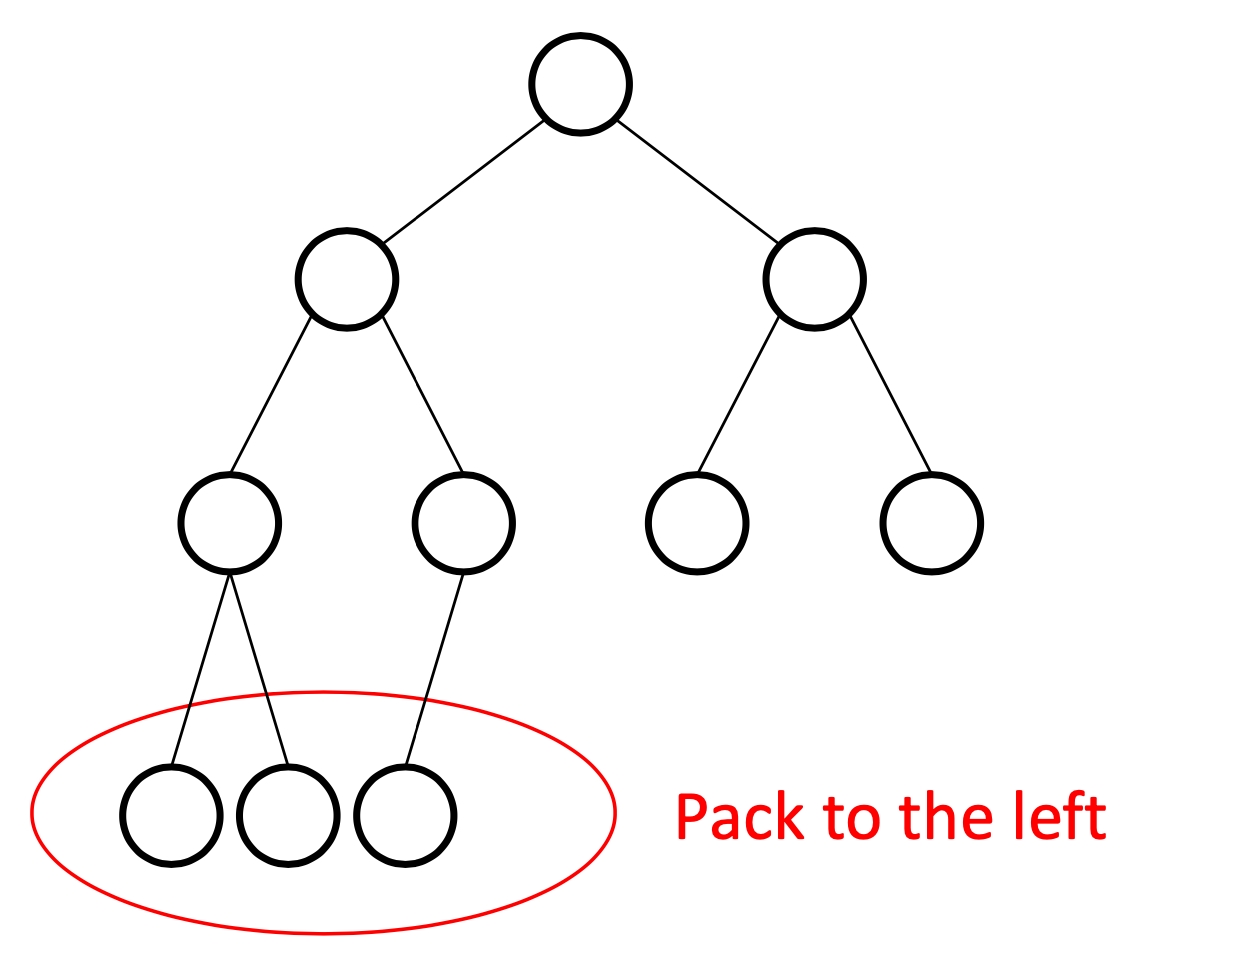
\includegraphics[scale=0.38]{images/05-heap-intro.png}
    \end{figure}

    We also define a special kind of heap called {\bf Min-heap}.
    \begin{definition}
        {\bf Min-heap} is a {\bf heap} in which the value of a node 
        is {\it at least} the value of its parent.
    \end{definition}
    \begin{figure}[htbp]
        \centering
        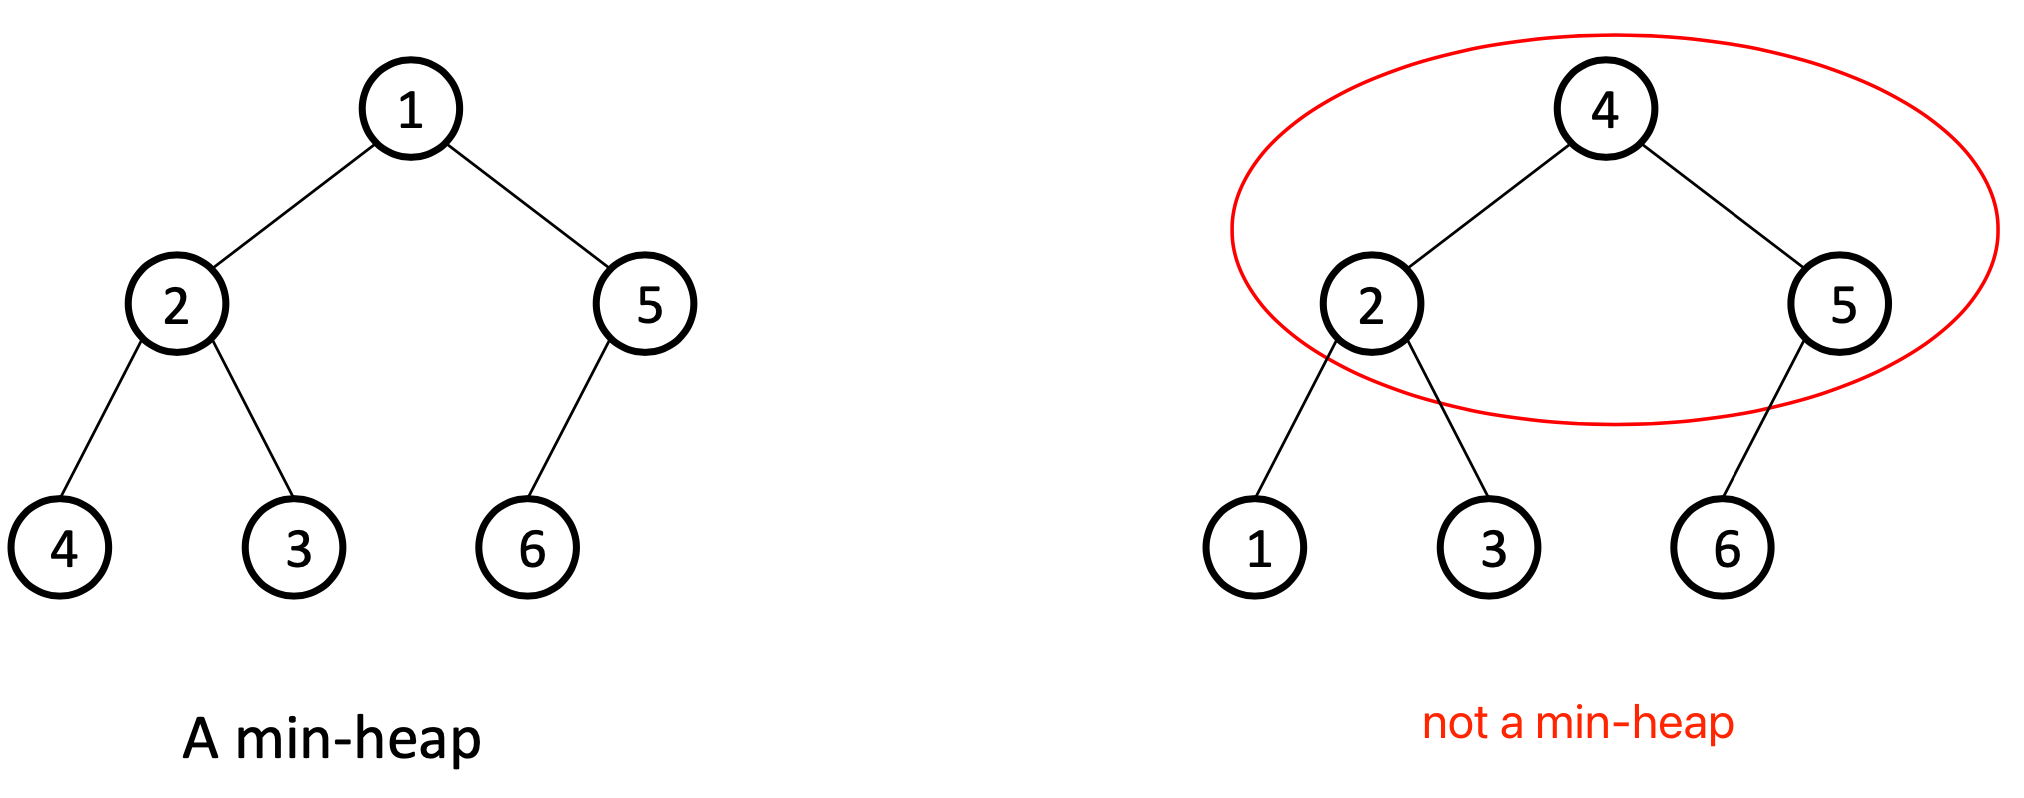
\includegraphics[scale=0.4]{images/05-min-heap-intro.png}
    \end{figure}

    Since {\bf heap} is a special kind of {\bf binary tree}, its height $h$
    and number of elements $n$ are related:
    \begin{theorem}
        For a {\bf heap} with $n$ elements and height $h$, there must be 
        $$2^h\le n<2^{h+1}$$
        thus an $n$-element heap has height $\Theta(\log n)$.
    \end{theorem}
    \begin{proof}
        The proof is trivial, only use the fact that a binary tree with height $h$
        can have at most $2^{h+1}-1$ nodes(height starts from 0), so a heap with 
        height $h$ must have $2^h-1$ nodes before level $h$(since they must be full).
    \end{proof}

    Interestingly, the structure of {\bf heap} is so regular so that we can 
    use an array to represent it.
    \begin{figure}[htbp]
        \centering
        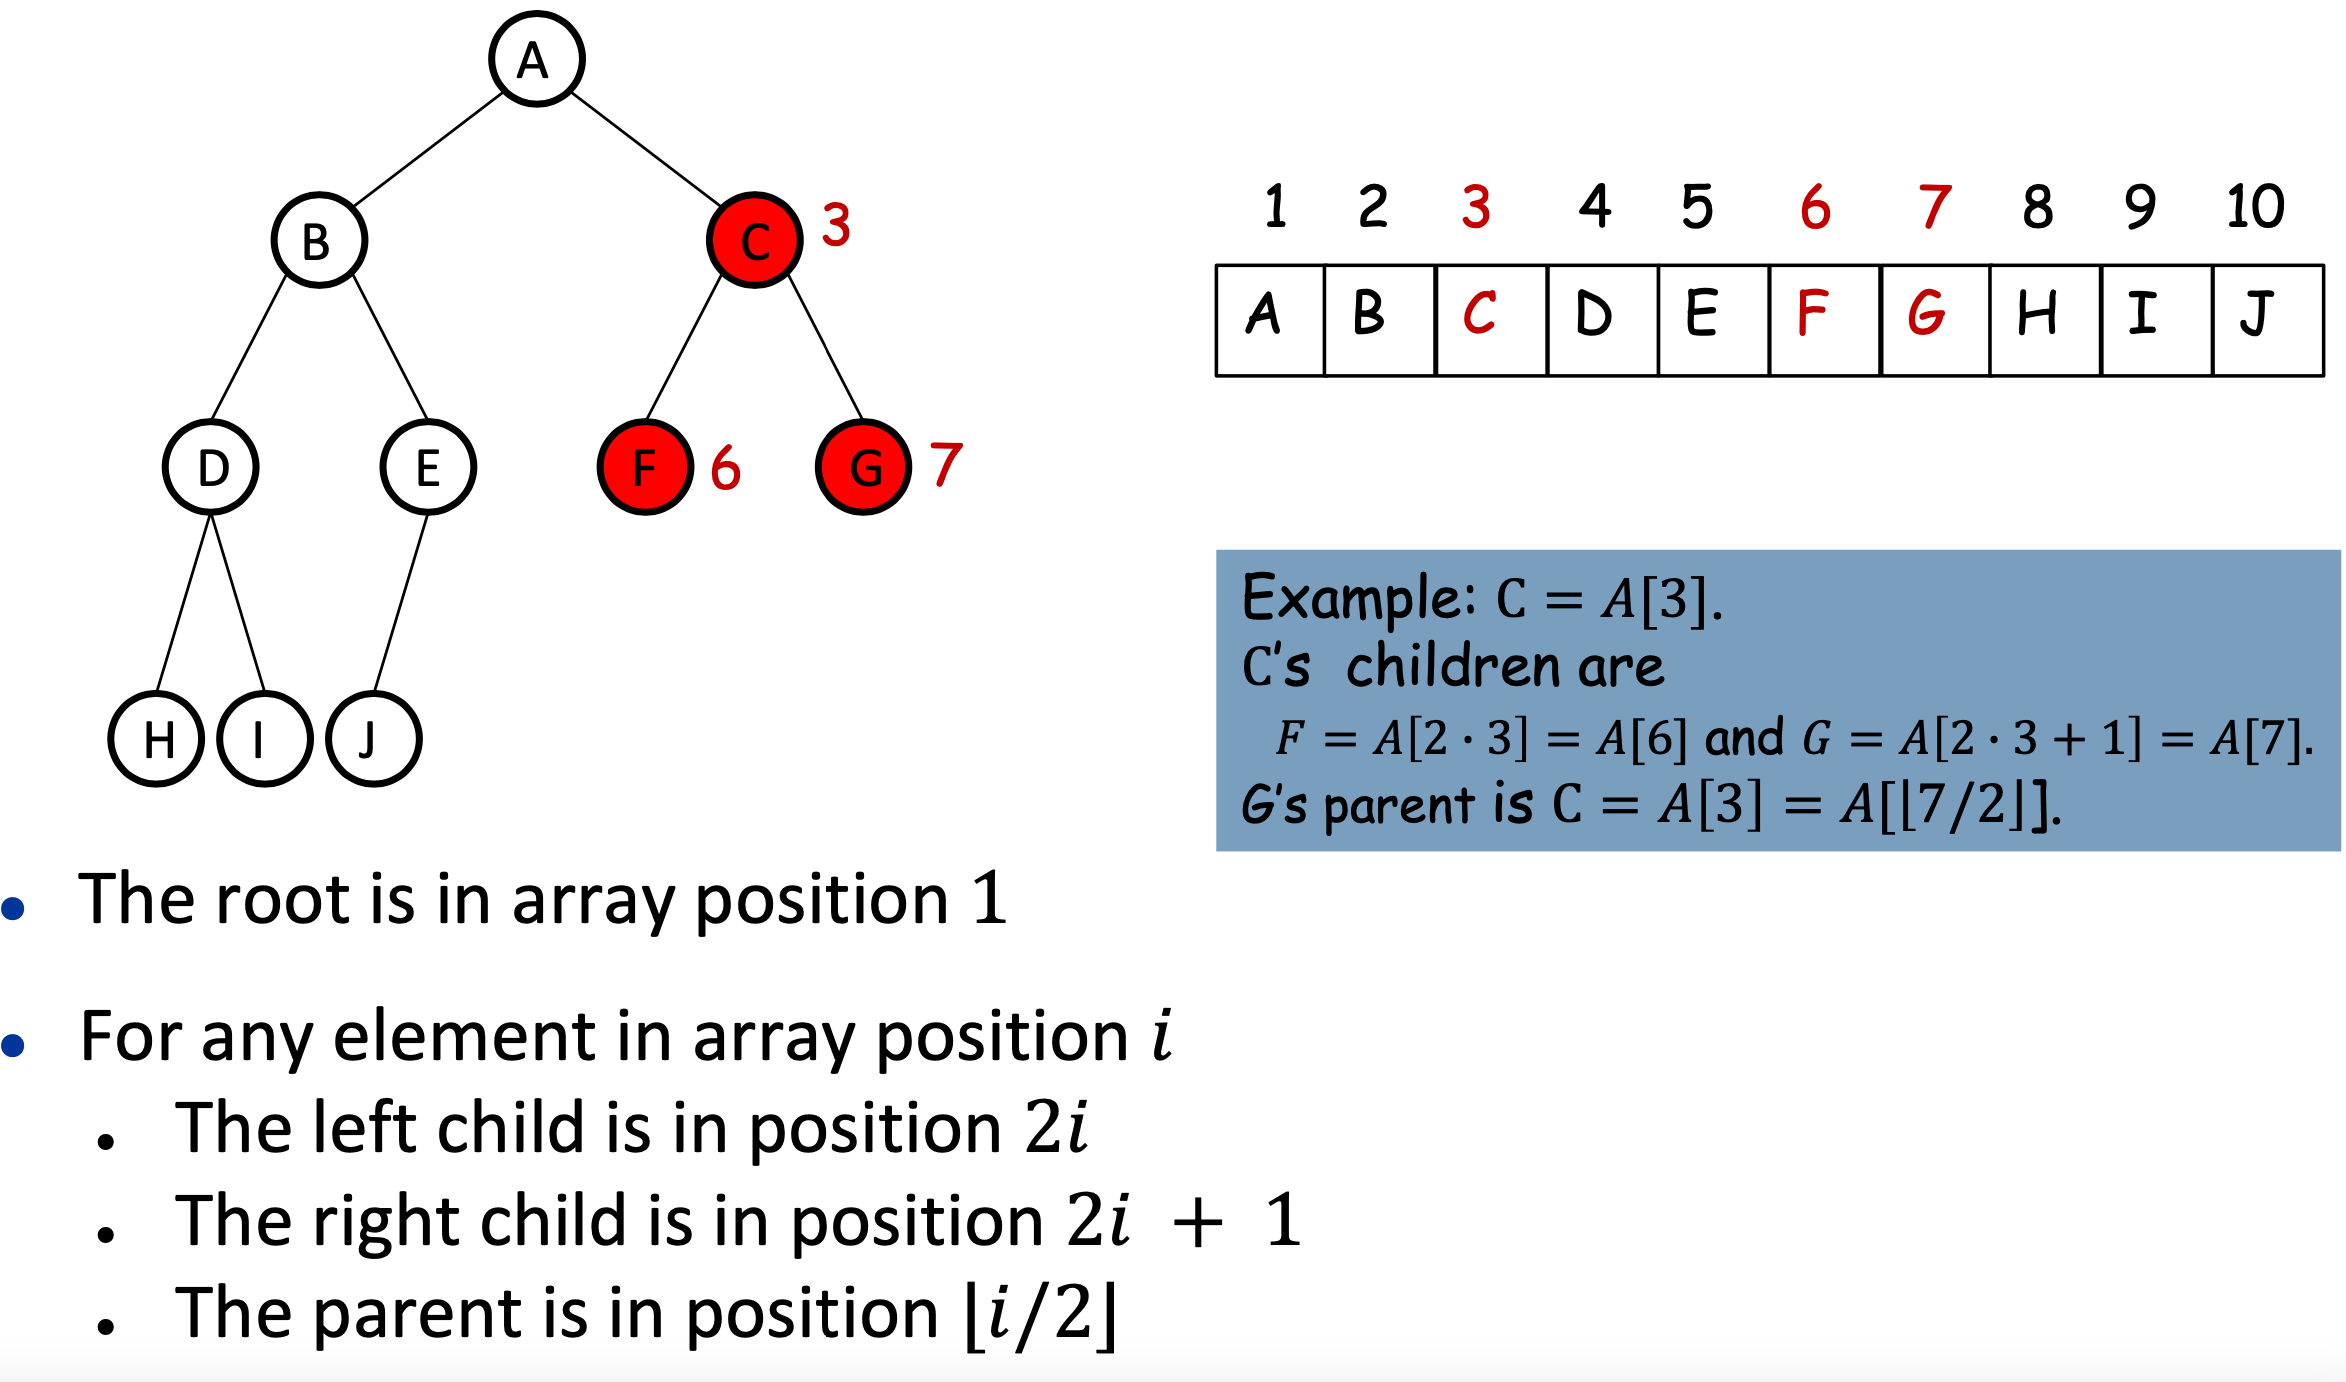
\includegraphics[scale=0.35]{images/05-heap-array.png}
    \end{figure}

    Now with the properties of heap, we can introduce how we can use heap to 
    efficiently perform {\bf insertion} and {\bf extract-min} operations.


    \vspace{0.3in}
    \section{Insertion}

    Recall that a heap must be ``left-packed'', so it is not surprising that 
    if we insert a new node, we should insert it into the {\it next available 
    position at the lowest level}. ``The lowest level'' is because the 
    upper levels are all full, and ``next available'' means the immediate 
    right position of the last node, which allows us to maintain the ``left-packed'' property.

    So if we insert 1 into the heap below, we end up with:
    \begin{figure}[htbp]
        \centering
        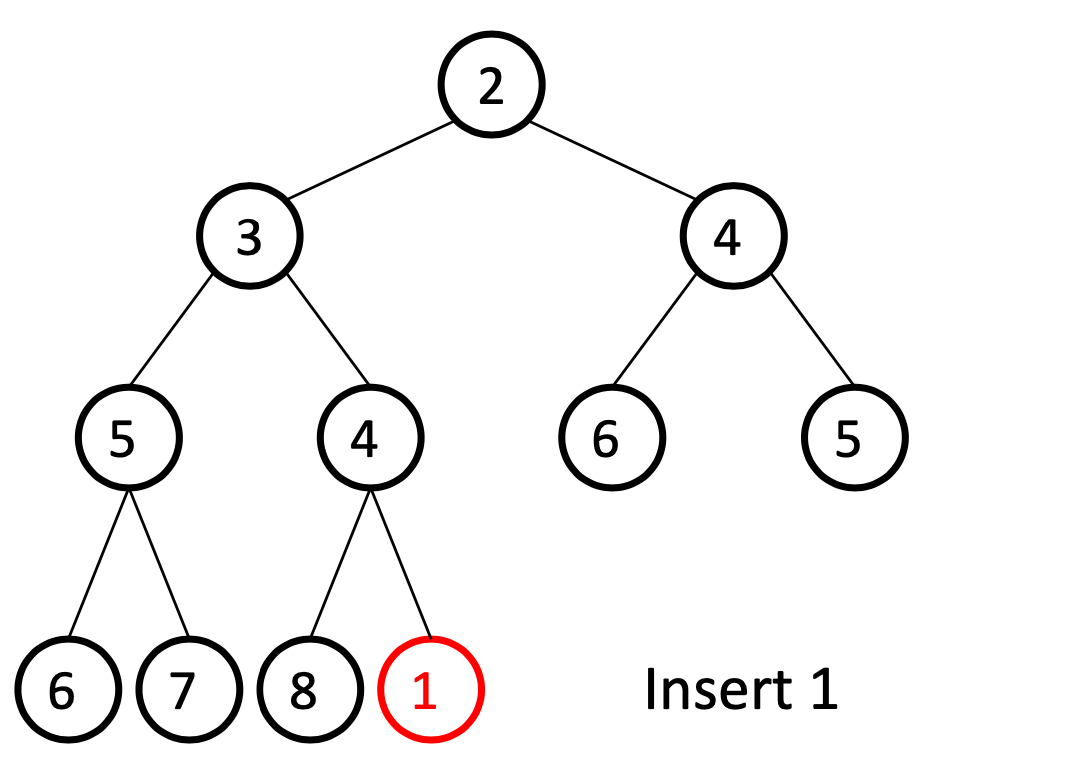
\includegraphics[scale=0.25]{images/05-insert-1.png}
    \end{figure}

    You may have already noticed that the new heap violates the ``min-heap property'', namely
    1 has a parent 4 that is larger than 1. To fix the problem, we consider 
    ``{\bf percolate up(or bubble up)}'': such that if the parent of the node is 
    larger than the node, we swap the parent with that child.

    Here, since $4>1$, we swap parent 4 and its child 1:
    \begin{figure}[htbp]
        \centering
        \qquad 
        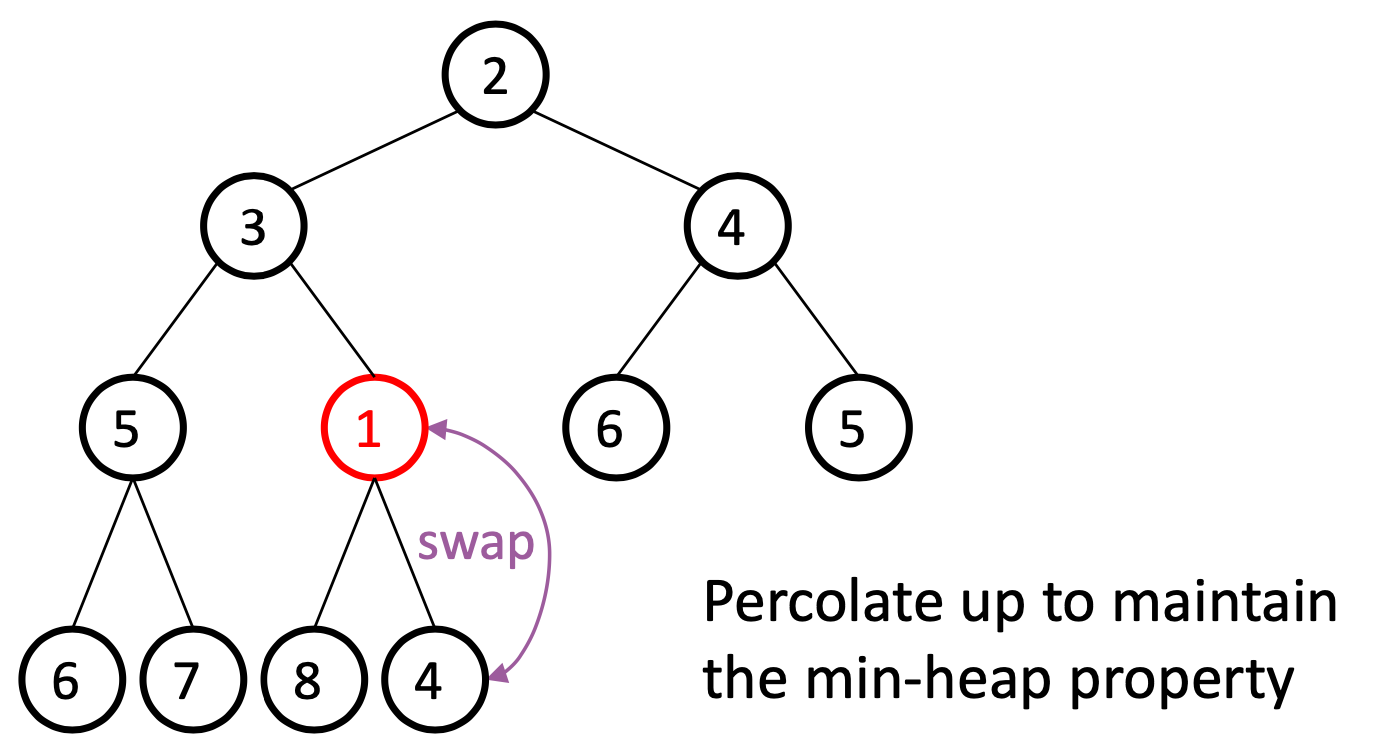
\includegraphics[scale=0.25]{images/05-insert-2.png}
    \end{figure}

    However, 1 still has a parent 3 that larger than 1, so we bubble up again:
    \begin{figure}[htbp]
        \centering
        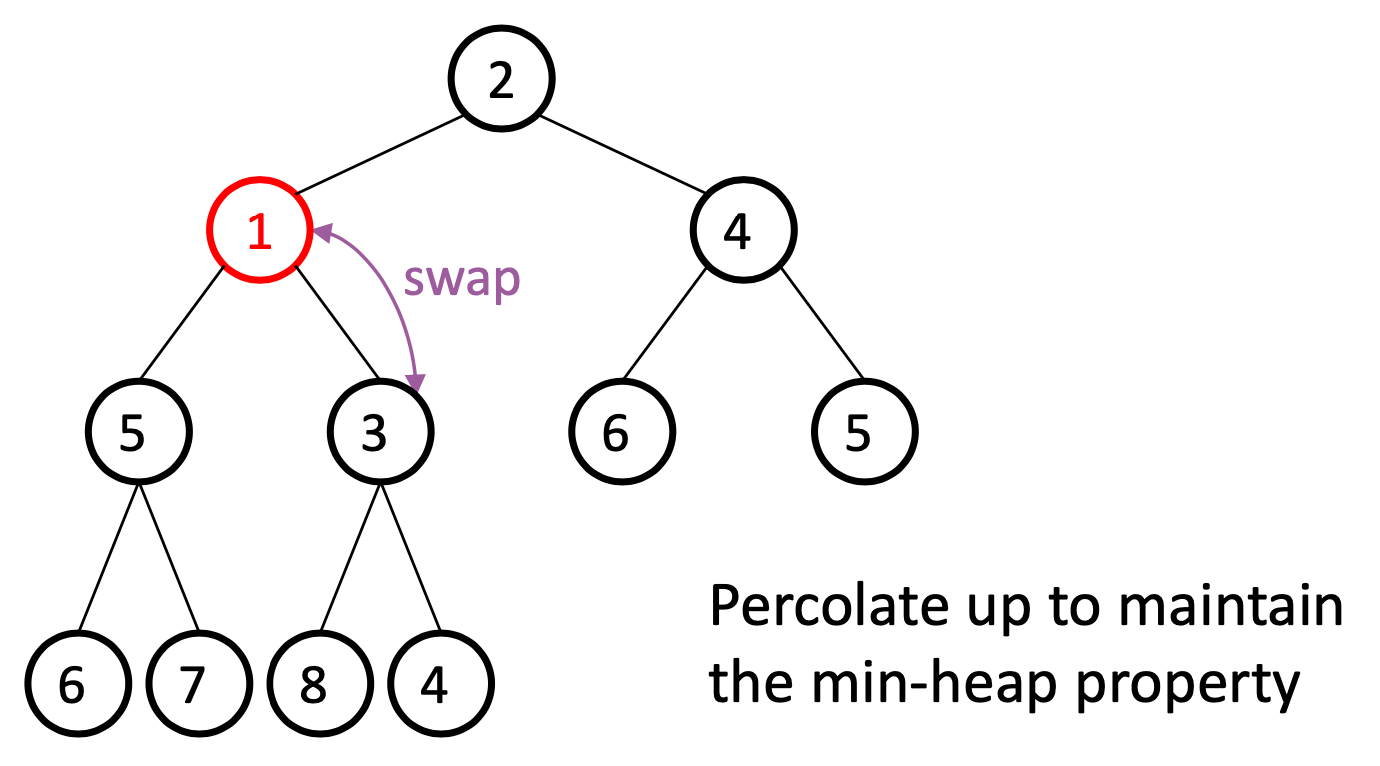
\includegraphics[scale=0.25]{images/05-insert-3.png}
    \end{figure}

    1 still has a parent 2 that larger than 1, bubble up again:
    \begin{figure}[htbp]
        \centering
        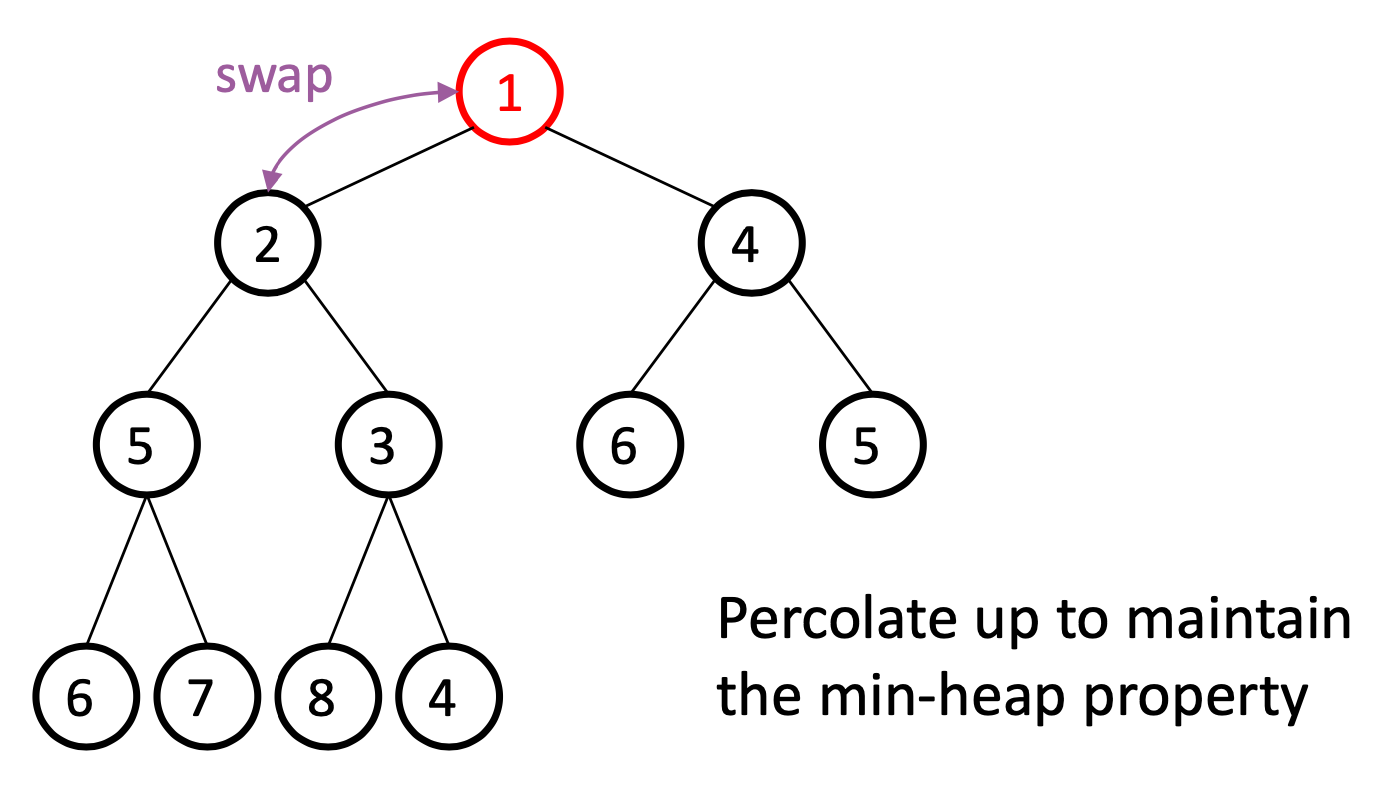
\includegraphics[scale=0.25]{images/05-insert-4.png}
    \end{figure}

    The heap now is fine.

    Since after each swap, the min-heap property is satisfied for the current subtree
    (with the new element as root), so after all those bubble up operations, the 
    min-heap property will certainly be preserved.

    The {\bf time complexity}, which can be measured by number of swaps, is 
    at most the height of heap, i.e., $O(\log n)$.

    We should notice that the swapping process is not necessarily stopped 
    when the new element reaching the top, instead, it stops when 
    its parent is smaller than it. For example, if we insert 2 into the resulted heap above,
    \begin{figure}[htbp]
        \centering
        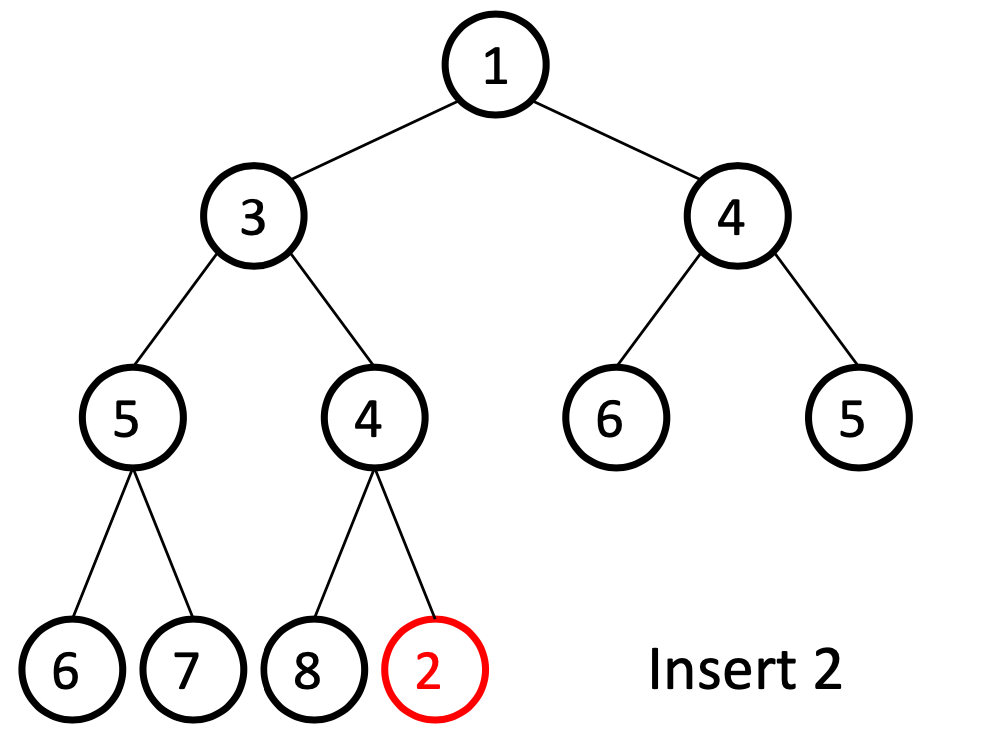
\includegraphics[scale=0.22]{images/05-insert-5.png}\quad 
        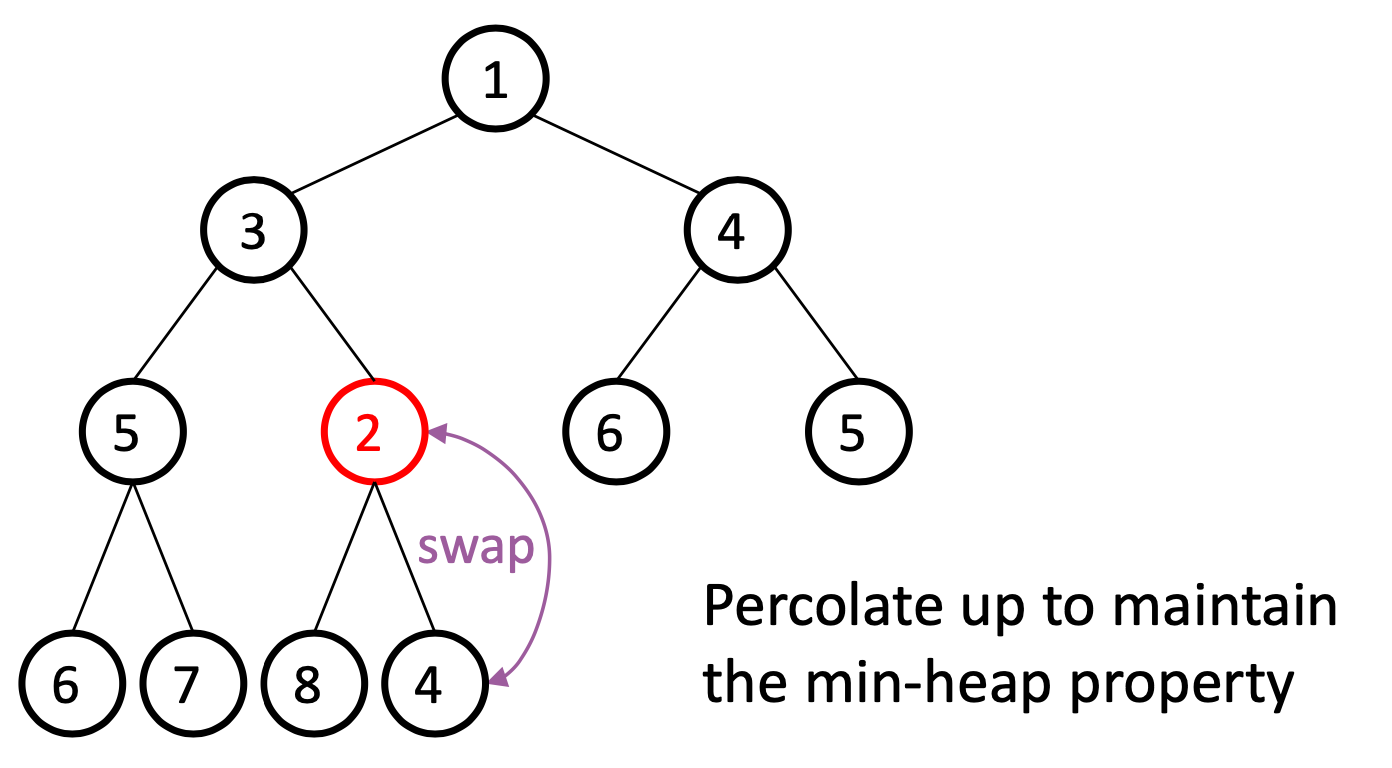
\includegraphics[scale=0.22]{images/05-insert-6.png}\quad 
        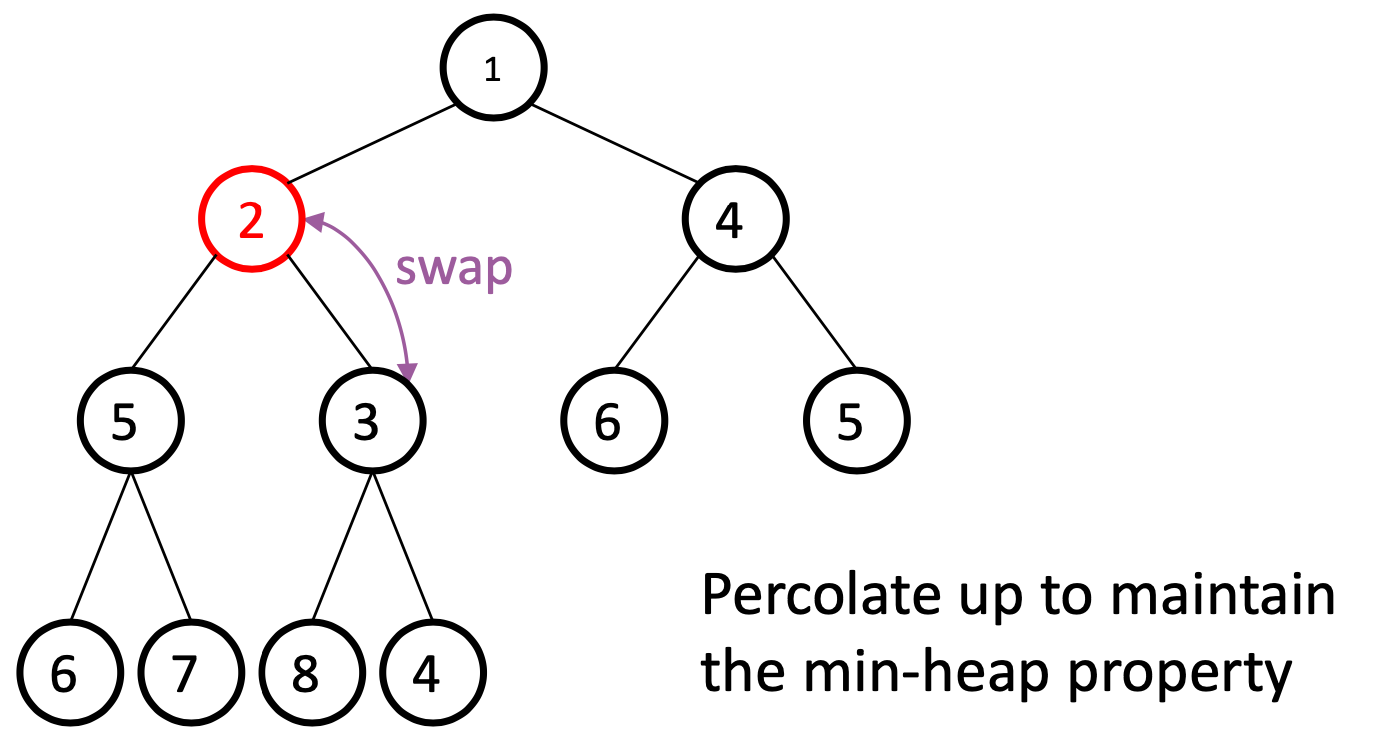
\includegraphics[scale=0.22]{images/05-insert-7.png}\quad 
    \end{figure}
    the process stops before reaching root 1.


    We conclude this section with pseudocode of Insert operation.
    \begin{algorithm*}[htbp]
        \caption{Insert($x$, $i$)}
        \tcp{Insert item $x$ to heap $A[1\cdots i-1]$ creating heap $A[1\cdots i]$}

        $A[i]\lar x$

        $j\lar i$

        \tcp{If smaller than parent, and not reach root yet}
        \While{$A[j]<A\left[\lf \frac{j}{2} \rf\right]$ and $j>1$}{
            \tcp{bubble up $A[j]$, swap with its parent}

            swap $A[j]$ and $A\left[\lf \frac{j}{2} \rf\right]$

            $j=\lf \frac{j}{2} \rf$\qquad \tcp{continue the process on new parent}
        }
    \end{algorithm*}

    \vspace{0.3in}
    \section{Extract-Min}

    Inspired by {\bf Insert} operation above, you may have already come up with 
    an idea that, we can remove the root(which is the min element), and then let 
    its children pop up. The image below shows the idea.
    \begin{figure}[htbp]
        \centering
        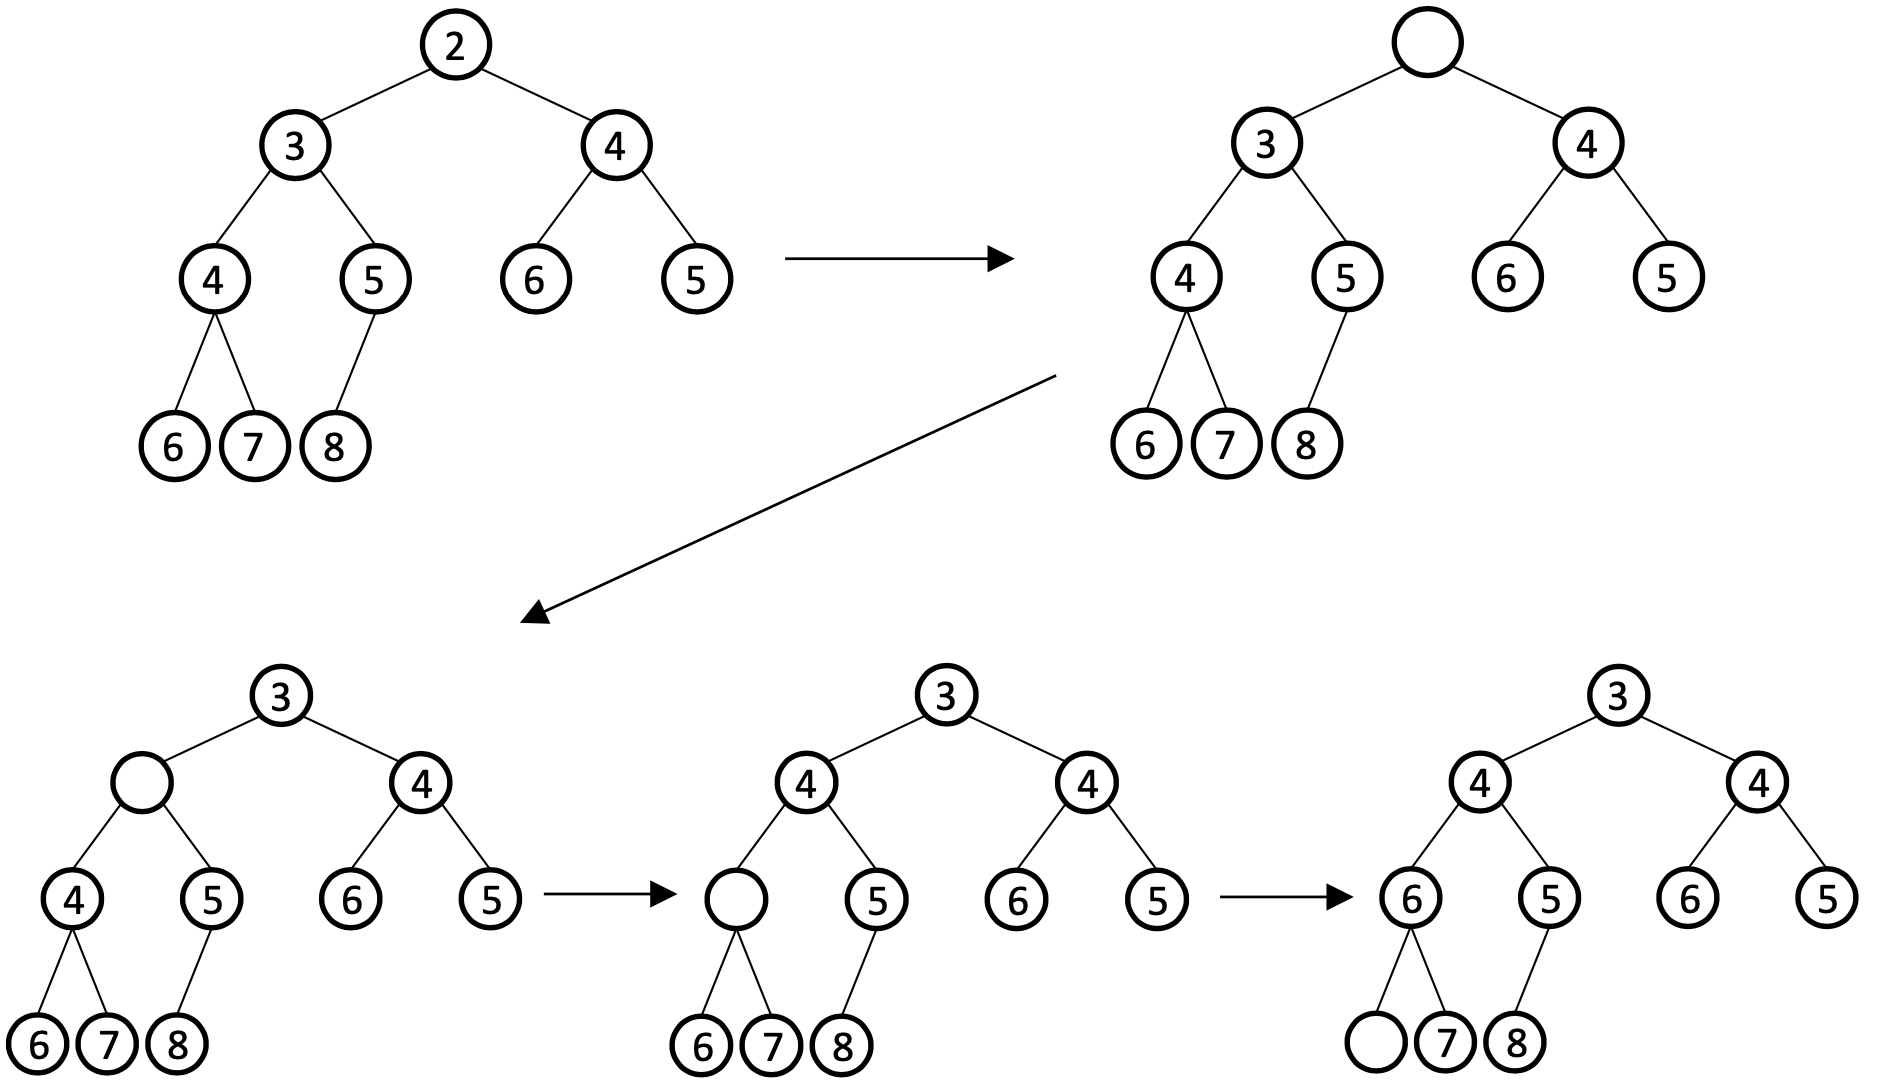
\includegraphics[scale=0.32]{images/05-min-wrong.png}
    \end{figure}

    As you may notice, the ``min-heap property'' is successfully preserved, however, 
    the result is no longer a heap: it is not ``left-packed''.

    In order to keep it ``left-packed'', we can only remove the right-most node 
    in lowest level. Therefore, we modify our previous idea into:
    \begin{itemize}
        \item Still, remove the root, which is the min element
        \item Then, let the right-most node in lowest level replace the original root
    \end{itemize}
    \begin{figure}[htbp]
        \centering
        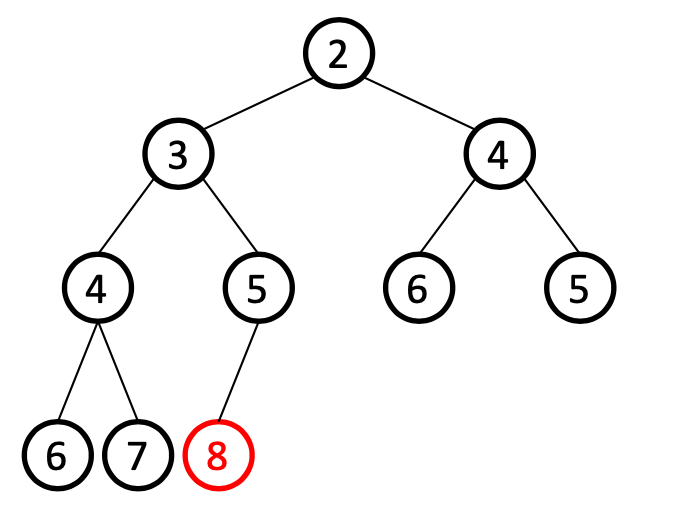
\includegraphics[scale=0.3]{images/05-min-1.png}\qquad 
        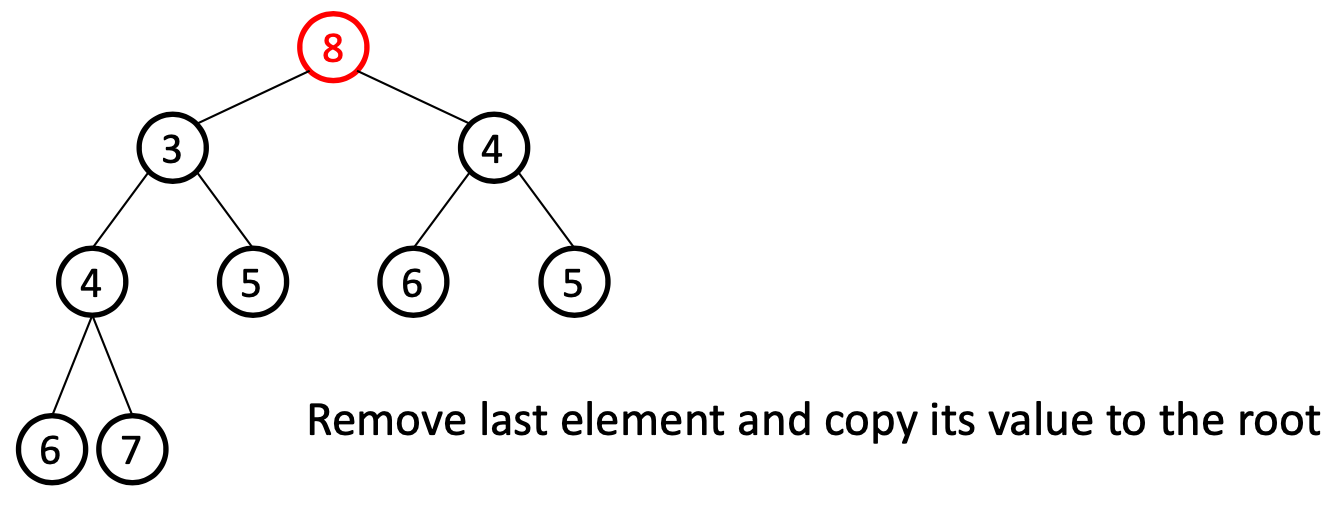
\includegraphics[scale=0.3]{images/05-min-2.png}
    \end{figure}

    By now, it only (possibly)violates the ``min-heap property'', and similar to what we've done 
    in {\bf Insert}, we can perform ``{\bf percolate down(or bubble down)}'', to 
    let the new root descent, until the ``min-heap property'' is satisfied.
    Notice that no matter how we bubble up/down, the shape of heap will not change,
    meaning that as long as the current heap is ``left-packed'', it will 
    still be ``left-packed'' after several bubble up/down operations.

    Use the same example above, we continue the process to bubble down new root:
    (notice that if the element is larger than both of its children, 
    we interchange it with the {\it smaller} children.)
    \begin{figure}[htbp]
        \centering
        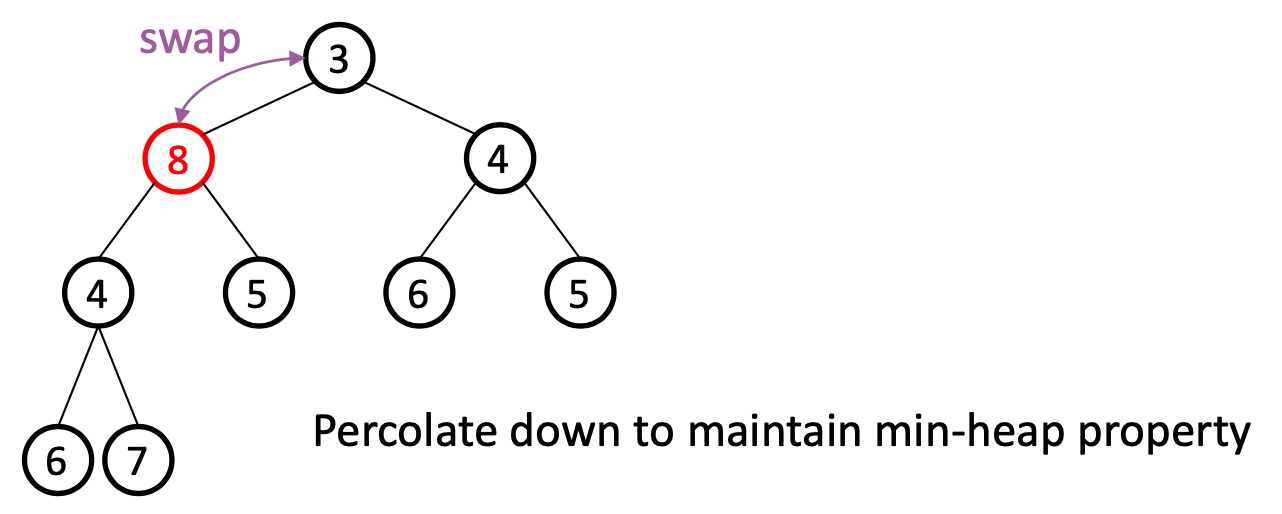
\includegraphics[scale=0.3]{images/05-min-3.png}\qquad
        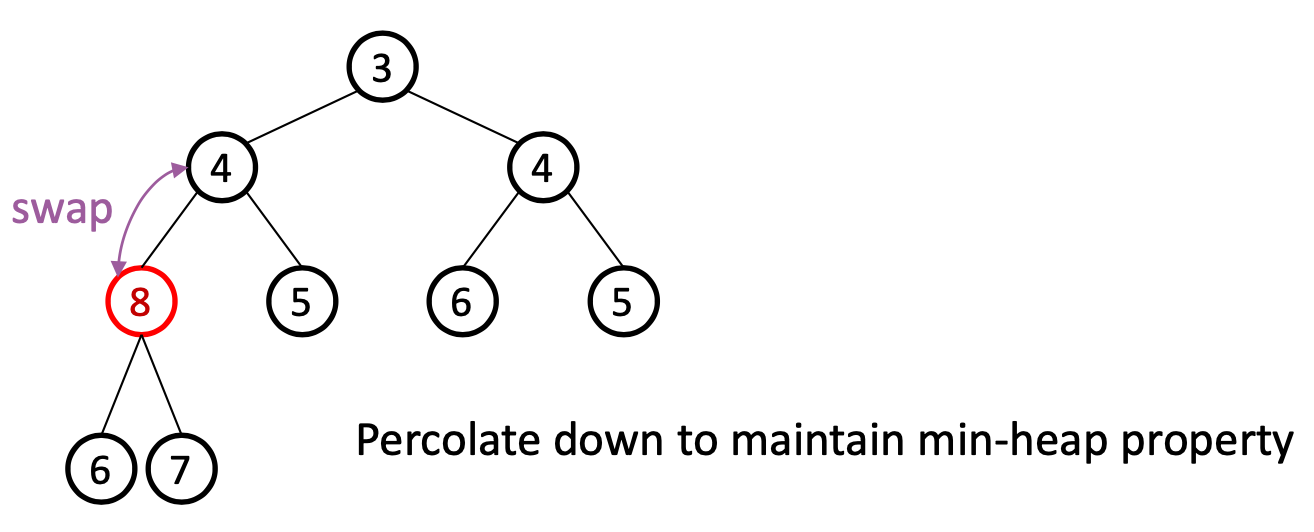
\includegraphics[scale=0.3]{images/05-min-4.png}\qquad 
        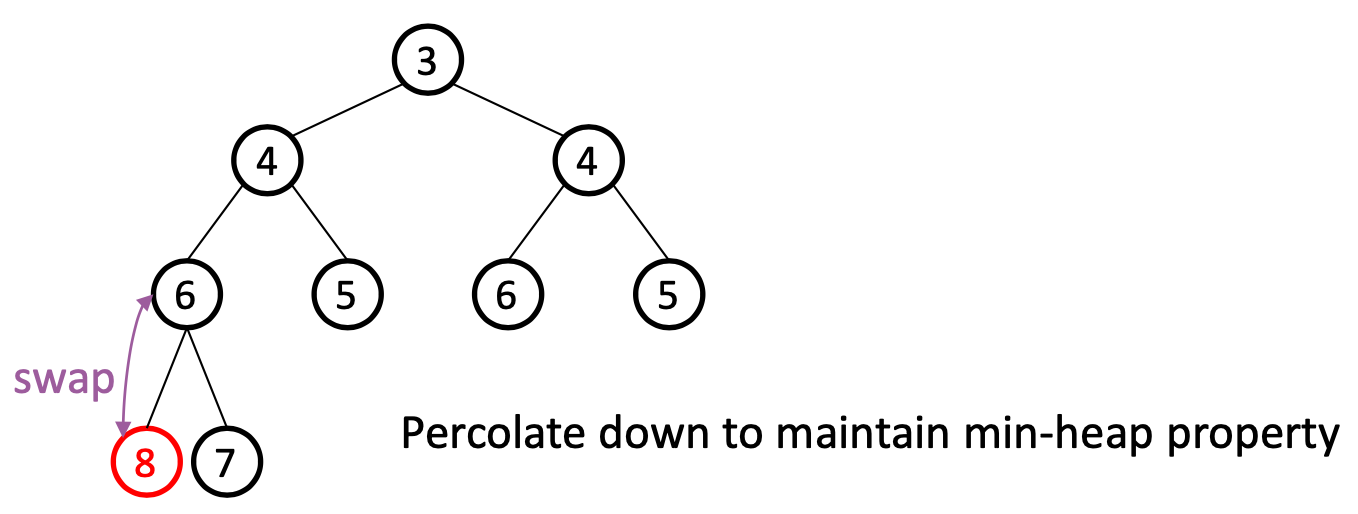
\includegraphics[scale=0.3]{images/05-min-5.png}
    \end{figure}
    
    The {\it correctness} can be verified in a similar manner as {\bf Insertion}:
    after each {\bf bubble down}, the min-heap property is satisfied for all
    nodes except the ``subtree'' containing the new root. And as we previously 
    mentioned, since the heap is ``left-packed'' before bubble down, 
    it will still be ``left-packed'' after those bubble operations.

    For {\it time complexity}, we still examine the number of swaps it performs,
    which at most, equals to the height of heap, i.e., $O(\log n)$.


    We ends up this section with the pseudocode of {\bf Extract-Min} operation.

    \begin{algorithm*}[htbp]
        \caption{Extract-Min($A[1\cdots i]$)}
        \tcp{Remove smallest item($A[i]$) in Heap, results in a new heap $A[1\cdots i-1]$}

        output($A[1]$) \qquad \tcp{$A[1]$ is the smallest one}

        swap $A[1]$ and $A[i]$\qquad \tcp{Let last element replace original root}

        $A[i]\lar nil$\qquad \tcp{Now $A[i]$ is empty}

        \tcp{Now we Bubble down from root}

        $j\lar 1,\ l\lar A[2j],\ r\lar A[2j+1]$ \qquad \tcp{$l,r$ are two children}
        \While{$A[j]>\min (l,r)$}{
            \tcp{Swap $A[j]$ with the smaller child }
            \eIf{$l<r$}{
                swap $A[j]$ with $A[2j]$

                $j\lar 2j$\qquad \tcp{contiuously bubble down}
            }{
                swap $A[j]$ with $A[2j+1]$

                $j\lar 2j+1$
            }
            $l\lar A[2j],\ r\lar A[2j+1]$\qquad \tcp{update values of two children for later bubble down}
        }
    \end{algorithm*}


    \vspace{0.3in}
    \section{Heap Sort}

    With the help of {\bf heap}, we can come up with a brand new sorting algorithm:
    \begin{itemize}
        \item Firstly, we {\bf Insert} $n$ elements one by one, which costs $O(n\log n)$
        \item Then, we perform $n$ {\bf Extract-Min} operations, which costs $O(n\log n)$ as well
        \item The elements we extracted above is sorted in ascending order.
    \end{itemize}

    So the total {\bf time complexity} for {\bf Heap Sort} is still $O(n\log n)$. 
    In tutorial, you will learn a cleverer method that can build a heap of $n$ elements 
    in $O(n)$, but this still cannot reduce the total running time.

    \vspace{0.3in}
    \section{Priority Queue}

    {\bf Priority Queue} is an abstract data structure that supports {\bf Insert} and 
    {\bf Extract-Min}, usually we consider priority queues are implemented using 
    heaps, so these two operations requires $O(\log n)$ time.

    Sometimes there is another operation {\bf Decrease-Key} supported in priority queues,
    which is useful when we talk about {\bf Dijkstra's Algorithm} for finding 
    Shortest Paths on a graph.

    \begin{definition}
        {\bf Decrease-Key:} decreases the value of one specified element.
    \end{definition}

    The way we implement {\bf Decrease-Key} is similar to previous operations, namely:
    \begin{itemize}
        \item Change the key of that node
        \item Continuously Bubble Up if necessary, until reaching root or ``min-heap property''
        holds.
    \end{itemize}
    We will not elaborate here.



\end{spacing}